\chapter{Inleiding}
\label{hoofdstuk:inleiding}

We zijn allemaal vertrouwd met afbeeldingen. Deze bestaan uit een 2D-rooster van pixels, waarbij elke pixel typisch bestaat uit drie kleurenwaarden die de intensiteit van rood, groen en blauw licht in de pixel beschrijven. Om deze reden zeggen we ook dat een normale afbeelding drie \textit{spectrale banden} bevat. Hiermee kan men het spectrum van zichtbaar licht goed benaderen op een manier die door het menselijk zicht waargenomen wordt op quasi identieke wijze als het originele beeld.\\

Voor sommige toepassingen is het echter ook nuttig om het gemeten lichtspectrum onder te verdelen in meer dan drie banden. In dit geval spreken we van \textit{hyperspectrale} afbeeldingen. Zo voert de AVIRIS-sensor (\textit{Airborne Visible/InfraRed Imaging Spectrometer}) van NASA \cite{ref:aviris_website} metingen uit in 224 banden over het zichtbare spectrum en een deel van het infrarood-spectrum. Toepassingen hiervan bestaan onder meer uit het opvolgen van de staat van landbouwgewassen \cite{ref:tilling}, het detecteren van afwijkingen in voedsel \cite{ref:higgins} en het in kaart brengen van mineralen op basis van luchtfoto's \cite{ref:resmini}.\\

Wanneer men hyperspectrale afbeeldingen wil opslaan, stoot men echter tegen een probleem. Een typische AVIRIS-dataset bevat miljoenen pixels en kan in een ongecomprimeerd formaat tientallen gigabytes groot zijn. Het is dus erg nuttig om compressietechnieken hiervoor te ontwikkelen.\\

In figuur \ref{fig:cuprite-bands} tonen we verschillende reeksen spectrale banden van een hyperspectrale luchtfoto van Cuprite (Nevada) in de Verenigde Staten. Er zijn significante verschillen zichtbaar tussen de banden, maar de structuur blijft duidelijk hetzelfde. Op spectraal niveau is er dus erg veel redundantie en dit kunnen we benutten om dezelfde data met minder geheugen voor te stellen.

\newpage
\begin{figure}[H]
\centering
\begin{subfigure}{0.48\textwidth}
  \centering
  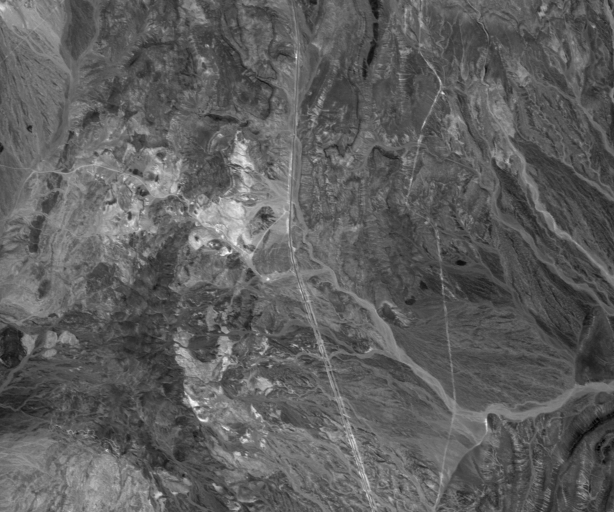
\includegraphics[width=0.95\linewidth]{images/cuprite_bands_0-32.png}
  \caption{Banden 0-31}
\end{subfigure}
\begin{subfigure}{0.48\textwidth}
  \centering
  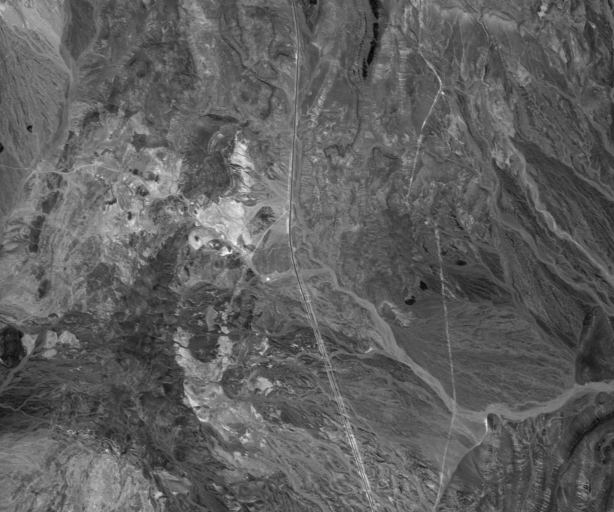
\includegraphics[width=0.95\linewidth]{images/cuprite_bands_32-63.png}
  \caption{Banden 32-62}
\end{subfigure}
\\
\begin{subfigure}{0.48\textwidth}
  \centering
  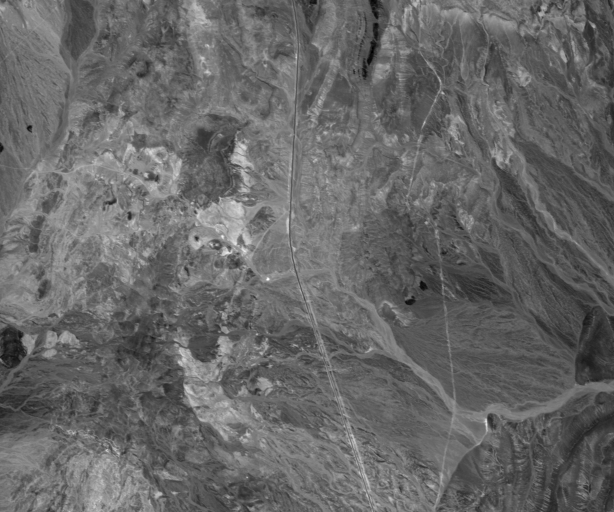
\includegraphics[width=0.95\linewidth]{images/cuprite_bands_63-95.png}
  \caption{Banden 63-94}
\end{subfigure}
\begin{subfigure}{0.48\textwidth}
  \centering
  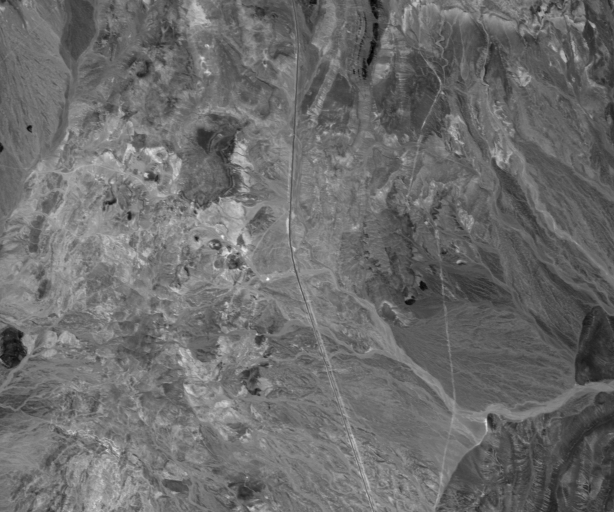
\includegraphics[width=0.95\linewidth]{images/cuprite_bands_95-127.png}
  \caption{Banden 95-126}
\end{subfigure}
\\
\begin{subfigure}{0.48\textwidth}
  \centering
  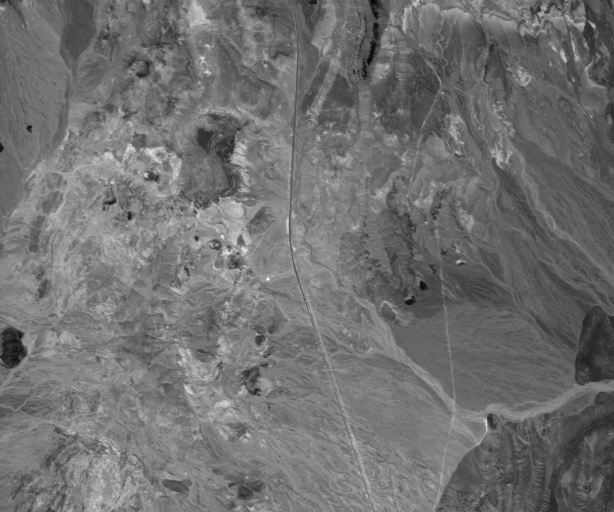
\includegraphics[width=0.95\linewidth]{images/cuprite_bands_127-158.png}
  \caption{Banden 127-157}
\end{subfigure}
\begin{subfigure}{0.48\textwidth}
  \centering
  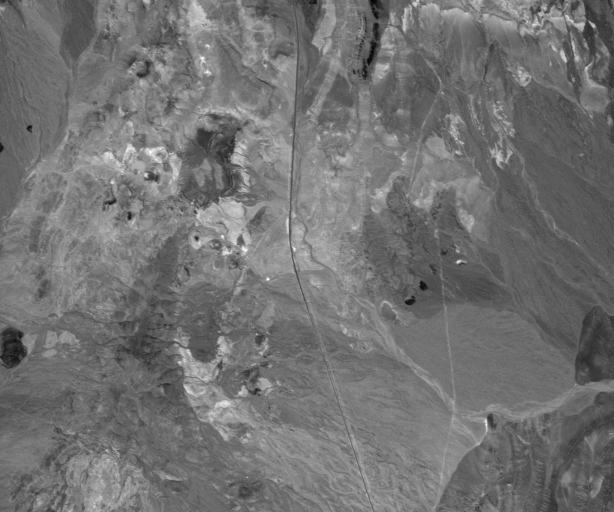
\includegraphics[width=0.95\linewidth]{images/cuprite_bands_158-190.png}
  \caption{Banden 158-189}
\end{subfigure}
\caption{Verschillende delen van een hyperspectrale afbeelding van Cuprite (VS) \cite{ref:ehu_aviris_cuprite}. We tonen hier slechts de 190 banden die overblijven na de voorverwerking die besproken zal worden in hoofdstuk \ref{hoofdstuk:methodologie}.}
\label{fig:cuprite-bands}
\end{figure}
\newpage

Wiskundig gezien kan men de 3D data van een hyperspectrale afbeelding beschouwen als een \textit{tensor}. Daarnaast kennen we vanuit de lineaire algebra de afgeknotte singulierewaardenontbinding, waarmee men met een beperkte fout matrices in een verkleind formaat kan opslaan. Aangezien men met deze decompositie effici\"ent de belangrijkste spectrale signaturen in een hyperspectrale afbeelding kan opsporen, zullen we in deze thesis compressie onderzoeken via tensordecomposities die hierop gebaseerd zijn.\\

Eerst zullen we in hoofdstuk \ref{hoofdstuk:achtergrond} enkele zaken herhalen en nieuwe concepten aanhalen zodat alle vereiste voorkennis besproken is. Het gaat hier onder andere over het verschil tussen \textit{lossless} en \textit{lossy} compressie, tensoren en hun operaties, de singulierewaardenontbinding en de Tucker-decompositie. Aan het einde van dit hoofdstuk volgt ook nog een korte literatuurstudie over hyperspectrale afbeeldingscompressie.\\

In hoofdstuk \ref{hoofdstuk:methodologie} bespreken we de methodologie achter de experimenten die we zullen uitvoeren in de volgende hoofdstukken. Daarna volgt hoofdstuk \ref{hoofdstuk:tucker} over compressie gebaseerd op de Tucker-decompositie, waarin het grootste deel van ons eigen onderzoek behandeld wordt. Hierin zullen we onderzoeken hoe we de singulierewaardenontbinding in bepaalde omstandigheden sneller kunnen berekenen, gevolgd door een analyse van de volgende stappen van de compressie: orthogonaliteitscompressie, quantisatie en encodering. Op deze manier bekomen we uiteindelijk een volledig Tucker-gebaseerd compressie-algoritme. Ten slotte bespreken we ook nog technieken om goede parameters te selecteren voor dit algoritme.\\

Hierna komt hoofdstuk \ref{hoofdstuk:hervorming}, waarin we de hyperspectrale afbeeldingen hervormen naar vijf dimensies en onderzoeken of er hiervoor betere compressiemethoden bestaan. We analyseren zowel het effect van Tucker-gebaseerde compressie als compressie gebaseerd op een nieuwe decompositie: \textit{tensor trains}.\\

In hoofdstuk \ref{hoofdstuk:resultaten} zullen we de uiteindelijke resultaten van onze compressiemethoden bespreken. Hierbij vergelijken we deze methoden zowel onderling als met enkele algemene compressie-algoritmen en een algoritme uit de literatuur, waarna we het hoofdstuk afsluiten met een aantal voorbeelden van gecomprimeerde hyperspectrale afbeeldingen.\\

Ten slotte eindigen we deze thesis met hoofdstuk \ref{hoofdstuk:besluit}, waarin we de conclusies van ons werk samenvatten. Hiernaast wordt er ook aandacht besteed aan mogelijke pistes voor verder onderzoek om onze compressie-algoritmen te verbeteren.